
%% bare_conf.tex
%% V1.3
%% 2007/01/11
%% by Michael Shell
%% See:
%% http://www.michaelshell.org/
%% for current contact information.
%%
%% This is a skeleton file demonstrating the use of IEEEtran.cls
%% (requires IEEEtran.cls version 1.7 or later) with an IEEE conference paper.
%%
%% Support sites:
%% http://www.michaelshell.org/tex/ieeetran/
%% http://www.ctan.org/tex-archive/macros/latex/contrib/IEEEtran/
%% and
%% http://www.ieee.org/

%%*************************************************************************
%% Legal Notice:
%% This code is offered as-is without any warranty either expressed or
%% implied; without even the implied warranty of MERCHANTABILITY or
%% FITNESS FOR A PARTICULAR PURPOSE! 
%% User assumes all risk.
%% In no event shall IEEE or any contributor to this code be liable for
%% any damages or losses, including, but not limited to, incidental,
%% consequential, or any other damages, resulting from the use or misuse
%% of any information contained here.
%%
%% All comments are the opinions of their respective authors and are not
%% necessarily endorsed by the IEEE.
%%
%% This work is distributed under the LaTeX Project Public License (LPPL)
%% ( http://www.latex-project.org/ ) version 1.3, and may be freely used,
%% distributed and modified. A copy of the LPPL, version 1.3, is included
%% in the base LaTeX documentation of all distributions of LaTeX released
%% 2003/12/01 or later.
%% Retain all contribution notices and credits.
%% ** Modified files should be clearly indicated as such, including  **
%% ** renaming them and changing author support contact information. **
%%
%% File list of work: IEEEtran.cls, IEEEtran_HOWTO.pdf, bare_adv.tex,
%%                    bare_conf.tex, bare_jrnl.tex, bare_jrnl_compsoc.tex
%%*************************************************************************

% *** Authors should verify (and, if needed, correct) their LaTeX system  ***
% *** with the testflow diagnostic prior to trusting their LaTeX platform ***
% *** with production work. IEEE's font choices can trigger bugs that do  ***
% *** not appear when using other class files.                            ***
% The testflow support page is at:
% http://www.michaelshell.org/tex/testflow/



% Note that the a4paper option is mainly intended so that authors in
% countries using A4 can easily print to A4 and see how their papers will
% look in print - the typesetting of the document will not typically be
% affected with changes in paper size (but the bottom and side margins will).
% Use the testflow package mentioned above to verify correct handling of
% both paper sizes by the user's LaTeX system.
%
% Also note that the "draftcls" or "draftclsnofoot", not "draft", option
% should be used if it is desired that the figures are to be displayed in
% draft mode.
%
\documentclass[10pt, conference, compsocconf]{IEEEtran}
% Add the compsocconf option for Computer Society conferences.
%
% If IEEEtran.cls has not been installed into the LaTeX system files,
% manually specify the path to it like:
% \documentclass[conference]{../sty/IEEEtran}





% Some very useful LaTeX packages include:
% (uncomment the ones you want to load)


% *** MISC UTILITY PACKAGES ***
%
%\usepackage{ifpdf}
% Heiko Oberdiek's ifpdf.sty is very useful if you need conditional
% compilation based on whether the output is pdf or dvi.
% usage:
% \ifpdf
%   % pdf code
% \else
%   % dvi code
% \fi
% The latest version of ifpdf.sty can be obtained from:
% http://www.ctan.org/tex-archive/macros/latex/contrib/oberdiek/
% Also, note that IEEEtran.cls V1.7 and later provides a builtin
% \ifCLASSINFOpdf conditional that works the same way.
% When switching from latex to pdflatex and vice-versa, the compiler may
% have to be run twice to clear warning/error messages.






% *** CITATION PACKAGES ***
%
%\usepackage{cite}
% cite.sty was written by Donald Arseneau
% V1.6 and later of IEEEtran pre-defines the format of the cite.sty package
% \cite{} output to follow that of IEEE. Loading the cite package will
% result in citation numbers being automatically sorted and properly
% "compressed/ranged". e.g., [1], [9], [2], [7], [5], [6] without using
% cite.sty will become [1], [2], [5]--[7], [9] using cite.sty. cite.sty's
% \cite will automatically add leading space, if needed. Use cite.sty's
% noadjust option (cite.sty V3.8 and later) if you want to turn this off.
% cite.sty is already installed on most LaTeX systems. Be sure and use
% version 4.0 (2003-05-27) and later if using hyperref.sty. cite.sty does
% not currently provide for hyperlinked citations.
% The latest version can be obtained at:
% http://www.ctan.org/tex-archive/macros/latex/contrib/cite/
% The documentation is contained in the cite.sty file itself.






% *** GRAPHICS RELATED PACKAGES ***
%
\ifCLASSINFOpdf
  % \usepackage[pdftex]{graphicx}
  % declare the path(s) where your graphic files are
  % \graphicspath{{../pdf/}{../jpeg/}}
  % and their extensions so you won't have to specify these with
  % every instance of \includegraphics
  % \DeclareGraphicsExtensions{.pdf,.jpeg,.png}
\else
  % or other class option (dvipsone, dvipdf, if not using dvips). graphicx
  % will default to the driver specified in the system graphics.cfg if no
  % driver is specified.
  % \usepackage[dvips]{graphicx}
  % declare the path(s) where your graphic files are
  % \graphicspath{{../eps/}}
  % and their extensions so you won't have to specify these with
  % every instance of \includegraphics
  % \DeclareGraphicsExtensions{.eps}
\fi
% graphicx was written by David Carlisle and Sebastian Rahtz. It is
% required if you want graphics, photos, etc. graphicx.sty is already
% installed on most LaTeX systems. The latest version and documentation can
% be obtained at: 
% http://www.ctan.org/tex-archive/macros/latex/required/graphics/
% Another good source of documentation is "Using Imported Graphics in
% LaTeX2e" by Keith Reckdahl which can be found as epslatex.ps or
% epslatex.pdf at: http://www.ctan.org/tex-archive/info/
%
% latex, and pdflatex in dvi mode, support graphics in encapsulated
% postscript (.eps) format. pdflatex in pdf mode supports graphics
% in .pdf, .jpeg, .png and .mps (metapost) formats. Users should ensure
% that all non-photo figures use a vector format (.eps, .pdf, .mps) and
% not a bitmapped formats (.jpeg, .png). IEEE frowns on bitmapped formats
% which can result in "jaggedy"/blurry rendering of lines and letters as
% well as large increases in file sizes.
%
% You can find documentation about the pdfTeX application at:
% http://www.tug.org/applications/pdftex





% *** MATH PACKAGES ***
%
%\usepackage[cmex10]{amsmath}
% A popular package from the American Mathematical Society that provides
% many useful and powerful commands for dealing with mathematics. If using
% it, be sure to load this package with the cmex10 option to ensure that
% only type 1 fonts will utilized at all point sizes. Without this option,
% it is possible that some math symbols, particularly those within
% footnotes, will be rendered in bitmap form which will result in a
% document that can not be IEEE Xplore compliant!
%
% Also, note that the amsmath package sets \interdisplaylinepenalty to 10000
% thus preventing page breaks from occurring within multiline equations. Use:
%\interdisplaylinepenalty=2500
% after loading amsmath to restore such page breaks as IEEEtran.cls normally
% does. amsmath.sty is already installed on most LaTeX systems. The latest
% version and documentation can be obtained at:
% http://www.ctan.org/tex-archive/macros/latex/required/amslatex/math/





% *** SPECIALIZED LIST PACKAGES ***
%
%\usepackage{algorithmic}
% algorithmic.sty was written by Peter Williams and Rogerio Brito.
% This package provides an algorithmic environment fo describing algorithms.
% You can use the algorithmic environment in-text or within a figure
% environment to provide for a floating algorithm. Do NOT use the algorithm
% floating environment provided by algorithm.sty (by the same authors) or
% algorithm2e.sty (by Christophe Fiorio) as IEEE does not use dedicated
% algorithm float types and packages that provide these will not provide
% correct IEEE style captions. The latest version and documentation of
% algorithmic.sty can be obtained at:
% http://www.ctan.org/tex-archive/macros/latex/contrib/algorithms/
% There is also a support site at:
% http://algorithms.berlios.de/index.html
% Also of interest may be the (relatively newer and more customizable)
% algorithmicx.sty package by Szasz Janos:
% http://www.ctan.org/tex-archive/macros/latex/contrib/algorithmicx/




% *** ALIGNMENT PACKAGES ***
%
%\usepackage{array}
% Frank Mittelbach's and David Carlisle's array.sty patches and improves
% the standard LaTeX2e array and tabular environments to provide better
% appearance and additional user controls. As the default LaTeX2e table
% generation code is lacking to the point of almost being broken with
% respect to the quality of the end results, all users are strongly
% advised to use an enhanced (at the very least that provided by array.sty)
% set of table tools. array.sty is already installed on most systems. The
% latest version and documentation can be obtained at:
% http://www.ctan.org/tex-archive/macros/latex/required/tools/


%\usepackage{mdwmath}
%\usepackage{mdwtab}
% Also highly recommended is Mark Wooding's extremely powerful MDW tools,
% especially mdwmath.sty and mdwtab.sty which are used to format equations
% and tables, respectively. The MDWtools set is already installed on most
% LaTeX systems. The lastest version and documentation is available at:
% http://www.ctan.org/tex-archive/macros/latex/contrib/mdwtools/


% IEEEtran contains the IEEEeqnarray family of commands that can be used to
% generate multiline equations as well as matrices, tables, etc., of high
% quality.


%\usepackage{eqparbox}
% Also of notable interest is Scott Pakin's eqparbox package for creating
% (automatically sized) equal width boxes - aka "natural width parboxes".
% Available at:
% http://www.ctan.org/tex-archive/macros/latex/contrib/eqparbox/





% *** SUBFIGURE PACKAGES ***
%\usepackage[tight,footnotesize]{subfigure}
% subfigure.sty was written by Steven Douglas Cochran. This package makes it
% easy to put subfigures in your figures. e.g., "Figure 1a and 1b". For IEEE
% work, it is a good idea to load it with the tight package option to reduce
% the amount of white space around the subfigures. subfigure.sty is already
% installed on most LaTeX systems. The latest version and documentation can
% be obtained at:
% http://www.ctan.org/tex-archive/obsolete/macros/latex/contrib/subfigure/
% subfigure.sty has been superceeded by subfig.sty.



%\usepackage[caption=false]{caption}
%\usepackage[font=footnotesize]{subfig}
% subfig.sty, also written by Steven Douglas Cochran, is the modern
% replacement for subfigure.sty. However, subfig.sty requires and
% automatically loads Axel Sommerfeldt's caption.sty which will override
% IEEEtran.cls handling of captions and this will result in nonIEEE style
% figure/table captions. To prevent this problem, be sure and preload
% caption.sty with its "caption=false" package option. This is will preserve
% IEEEtran.cls handing of captions. Version 1.3 (2005/06/28) and later 
% (recommended due to many improvements over 1.2) of subfig.sty supports
% the caption=false option directly:
%\usepackage[caption=false,font=footnotesize]{subfig}
%
% The latest version and documentation can be obtained at:
% http://www.ctan.org/tex-archive/macros/latex/contrib/subfig/
% The latest version and documentation of caption.sty can be obtained at:
% http://www.ctan.org/tex-archive/macros/latex/contrib/caption/




% *** FLOAT PACKAGES ***
%
%\usepackage{fixltx2e}
% fixltx2e, the successor to the earlier fix2col.sty, was written by
% Frank Mittelbach and David Carlisle. This package corrects a few problems
% in the LaTeX2e kernel, the most notable of which is that in current
% LaTeX2e releases, the ordering of single and double column floats is not
% guaranteed to be preserved. Thus, an unpatched LaTeX2e can allow a
% single column figure to be placed prior to an earlier double column
% figure. The latest version and documentation can be found at:
% http://www.ctan.org/tex-archive/macros/latex/base/



%\usepackage{stfloats}
% stfloats.sty was written by Sigitas Tolusis. This package gives LaTeX2e
% the ability to do double column floats at the bottom of the page as well
% as the top. (e.g., "\begin{figure*}[!b]" is not normally possible in
% LaTeX2e). It also provides a command:
%\fnbelowfloat
% to enable the placement of footnotes below bottom floats (the standard
% LaTeX2e kernel puts them above bottom floats). This is an invasive package
% which rewrites many portions of the LaTeX2e float routines. It may not work
% with other packages that modify the LaTeX2e float routines. The latest
% version and documentation can be obtained at:
% http://www.ctan.org/tex-archive/macros/latex/contrib/sttools/
% Documentation is contained in the stfloats.sty comments as well as in the
% presfull.pdf file. Do not use the stfloats baselinefloat ability as IEEE
% does not allow \baselineskip to stretch. Authors submitting work to the
% IEEE should note that IEEE rarely uses double column equations and
% that authors should try to avoid such use. Do not be tempted to use the
% cuted.sty or midfloat.sty packages (also by Sigitas Tolusis) as IEEE does
% not format its papers in such ways.





% *** PDF, URL AND HYPERLINK PACKAGES ***
%
%\usepackage{url}
% url.sty was written by Donald Arseneau. It provides better support for
% handling and breaking URLs. url.sty is already installed on most LaTeX
% systems. The latest version can be obtained at:
% http://www.ctan.org/tex-archive/macros/latex/contrib/misc/
% Read the url.sty source comments for usage information. Basically,
% \url{my_url_here}.





% *** Do not adjust lengths that control margins, column widths, etc. ***
% *** Do not use packages that alter fonts (such as pslatex).         ***
% There should be no need to do such things with IEEEtran.cls V1.6 and later.
% (Unless specifically asked to do so by the journal or conference you plan
% to submit to, of course. )


% correct bad hyphenation here
\hyphenation{op-tical net-works semi-conduc-tor}

\usepackage{listings}
\usepackage{graphicx}
\usepackage{amsmath}
%\linespread{2}
%\linespread{0.99}

\begin{document}
%
% paper title
% can use linebreaks \\ within to get better formatting as desired
\title{A Novel High-Throughput Acceleration Engine for Read Alignment}


% author names and affiliations
% use a multiple column layout for up to two different
% affiliations

\author{\IEEEauthorblockN{Yu-ting Chen, Jason Cong, Peng Wei}
\IEEEauthorblockA{Computer Science Department\\
University of California, Los Angeles\\
Los Angeles, CA, 90095, USA\\
{ytchen, cong, peng.wei.prc}@cs.ucla.edu}
\and
\IEEEauthorblockN{Jie Lei}
\IEEEauthorblockA{State Key Laboratory of Integrated Services Networks\\
Xidian University\\
Xian, China\\
jielei@mail.xidian.edu.cn}
}

% conference papers do not typically use \thanks and this command
% is locked out in conference mode. If really needed, such as for
% the acknowledgment of grants, issue a \IEEEoverridecommandlockouts
% after \documentclass

% for over three affiliations, or if they all won't fit within the width
% of the page, use this alternative format:
% 
%\author{\IEEEauthorblockN{Michael Shell\IEEEauthorrefmark{1},
%Homer Simpson\IEEEauthorrefmark{2},
%James Kirk\IEEEauthorrefmark{3}, 
%Montgomery Scott\IEEEauthorrefmark{3} and
%Eldon Tyrell\IEEEauthorrefmark{4}}
%\IEEEauthorblockA{\IEEEauthorrefmark{1}School of Electrical and Computer Engineering\\
%Georgia Institute of Technology,
%Atlanta, Georgia 30332--0250\\ Email: see http://www.michaelshell.org/contact.html}
%\IEEEauthorblockA{\IEEEauthorrefmark{2}Twentieth Century Fox, Springfield, USA\\
%Email: homer@thesimpsons.com}
%\IEEEauthorblockA{\IEEEauthorrefmark{3}Starfleet Academy, San Francisco, California 96678-2391\\
%Telephone: (800) 555--1212, Fax: (888) 555--1212}
%\IEEEauthorblockA{\IEEEauthorrefmark{4}Tyrell Inc., 123 Replicant Street, Los Angeles, California 90210--4321}}




% use for special paper notices
%\IEEEspecialpapernotice{(Invited Paper)}




% make the title area
\maketitle


\begin{abstract}
The Smith-Waterman (S-W) algorithm is widely adopted by the state-of-the-art DNA sequece aligners.
Existing wavefront-based works for accelerating S-W ignored the fact that S-W is called with significantly varied input sizes and extensive pruning in modern aligners. 
In this paper, we propose an architecture, 
tailored for varied input sizes as well as harnessing software pruning strategies, 
to accelerate S-W. 
Our implementation demonstrates 26.4x speedup over a 24-thread Intel Haswell Xeon server, 
and outperforms wavefront-based implementations up to 6x with the same FPGA resource.
%%%
%%%Next-generation sequencing is one of the most burgeoning technologies for biological research and clinical applications.
%%%A sequencer generates billions of reads collected from a single human sample.
%%%These reads need to be aligned to the human reference genome for further analysis.
%%%The state-of-the-art read aligners, such as BWA-MEM and Bowtie 2, use an extended Smith-Waterman (S-W) algorithm, which is compute-intensive, to perform read alignment. 
%%%While prior works have successfully accelerated the stand-alone classic S-W algorithm on FPGAs by exploiting the anti-diagonal parallelism, 
%%%they ignored the complexity of how to integrate the S-W algorithm into modern read aligners,  
%%%where the S-W algorithm is called with significantly varied input sizes, and extensive pruning is performed in the S-W algorithm.
%%%As a result, existing FPGA accelerators for the S-W algorithm are difficult and ineffective when integrated in the modern aligners.
%%%In this paper, we propose a novel architecture realized on FPGA to accelerate the extended S-W algorithm.
%%%The architecture achieves better performance than existing wavefront-based acceleration solutions when encountering significantly varied input sizes,
%%%as well as achieves further speedup by fully utilizing software pruning strategies for hardware acceleration.
%%%Compared to a 24-thread Intel Haswell Xeon server, our FPGA implementation demonstrates 26.4x speedup.
%%%We also show that our design outperforms wavefront-based implementations up to 6x with the same FPGA resource.
\end{abstract}

\begin{IEEEkeywords}
read alignment; Smith-Waterman; FPGA; HLS; multi-level scheduling
\end{IEEEkeywords}
% For peer review papers, you can put extra information on the cover
% page as needed:
% \ifCLASSOPTIONpeerreview
% \begin{center} \bfseries EDICS Category: 3-BBND \end{center}
% \fi
%
% For peerreview papers, this IEEEtran command inserts a page break and
% creates the second title. It will be ignored for other modes.
\IEEEpeerreviewmaketitle
\section{Introduction} 
\label{sec:introduction}

Next-generation sequencing (NGS) technologies have attracted a large amount of attention from both researchers and clinicians. 
Human DNA samples are chopped into billions of small fragments, called reads, and a sequencer determines the order of each read's nucleotides. 
A software aligner then maps the billions of sequenced reads onto a reference human genome, which entails tremendous computational challenges.
%%%The size of a DNA sequence is often measured in base pairs (bps). 
A read typically consists of hundreds of nucleotides or base pairs (bps), while the reference genome contains 3.2 billion bps \cite{Mardis2008}.
%%The advent of next-generation sequencing (NGS) technologies dramatically reduces the cost of genome sequencing. 
%%Today's sequencing technologies can obtain a genome for an individual for \$1,000 or less \cite{Mardis2006}. 
%%The technology can be widely used in research and is transitioning into the clinic for applications such as precision medicine for cancer treatment. 
%%Next-generation sequencers are more cost-effective because they generate the sequence 
%%from very small fragments (reads) of length in the range of a few hundred nucleotides. 
%%Mapping billions of sequenced fragments onto a genome sequence by taking advantage of the known human genome sequence 
%%is called resequencing, and it entails tremendous computational challenges.

State-of-the-art read aligners, such as BWA-MEM \cite{BWA-MEM} and Bowtie 2 \cite{Bowtie2}, 
carry out the read mapping in two steps. 
First, each read is fragmented into small pieces called seeds, and mapped to the reference genome. 
The mapping of seeds to the reference genome must be exact, i.e., no gap or mismatch is allowed. 
A backward search algorithm based on the Burrows-Wheeler Transform (BWT) \cite{BWT} takes only O($m$) time for a seed of length $m$ to map to the super-long reference genome, independent of the size of the reference genome, and therefore is employed by almost all contemporary sequence aligners.

In the second step, each seed map gets extended leftward and rightward to span the entire read. 
The extensions allow inexact mappings, in which gaps and mismatches are allowed. A predefined scoring function is provided for evaluating the effectiveness of inexact mappings. Only the ones achieving high enough scores are recorded in the output. 
The Smith-Waterman (S-W) algorithm, a dynamic programming (DP) algorithm with quadratic time complexity, is a commonly used approach to address this problem. 
It is the main computation bottleneck in state-of-the-art tools like BWA-MEM \cite{BWA-MEM} (taking 30\%~50\% computation time). 
In this work we focus on accelerating the S-W algorithm in BWA-MEM. The methodology, however, can be applied to other contemporary aligners, such as Bowtie 2 \cite{Bowtie2} and LAST \cite{LAST}. 

The S-W algorithm is inherently anti-diagonal parallelizable, since the elements along the anti-diagonal direction in the 2D table used during the DP procedure are independent of each other \cite{Edmiston1988}. 
This feature, called wavefront, has been explored in different ways on different platforms \cite{Preusser2012}\cite{RaceLogic}\cite{Zhang2007}\cite{Lam2013}. 
It works fairly well when inputs are homogeneous. 
However, the solutions that target the general S-W algorithm do not fit very well for the optimized version used in BWA-MEM. 
First, a huge number of reads at the billion scale need to be processed with high throughput. 
Conventional approaches may result in an overemphasis on inner-task parallelism. 
Second, conventional wavefront-based architectures cannot utilize computational resources efficiently when the input sizes vary sharply, as in BWA-MEM. 
Third, the pruning heuristic used in BWA-MEM prevents conventional solutions from being adopted directly and efficiently.

In this paper, we propose an architecture to address these issues.
The novelties of our architecture can be summarized as follows: 
(1) We propose an array-based architecture for processing the enormous number of reads in a high-throughput fashion, adapting better to inputs with widely varied sizes. 
(2) We provide a two-level hierarchical architecture for resource management, avoiding wasting resources in synthesizing bus interfaces while satisfying the off-chip bandwidth demand.
(3) Our design supports the pruning technique, shortening the runtime of S-W significantly. 

Our FPGA implementation demonstrates a 26.4x speedup compared to a 24-thread Intel Haswell Xeon server for the S-W kernel in BWA-MEM. 
We also show that our design outperforms wavefront-based implementations by up to 6x with the same FPGA resource utilization.

%%%\section{Background and Motivation} 
\label{sec:motivation}

\subsection{The General Smith-Waterman (S-W) Algorithm}
\label{subsec:general_SW}

As a fundamental operation in computational genetics, 
the acceleration of the general S-W algorithm has attracted a large amount of attention from academia \cite{Aluru2014}. 
The general S-W algorithm is anti-diagonal parallelizable, 
since the elements along each anti-diagonal in the S-W matrix are independent of each other, 
and each element only depends on three elements from the previous two anti-diagonals \cite{Edmiston1988}. 
Therefore, the wavefront property, as illustrated in Figure \ref{fig:F3C2}, 
has been used by researchers in almost all kinds of platforms for the S-W algorithm acceleration \cite{Wozniak1997}\cite{Arram2013}\cite{Preusser2012}\cite{Olson2012}\cite{RaceLogic}.
%REF achieves significant speedup with the anti-diagonal parallelism well-explored.
\begin{figure}[!hbt]
	\begin{center}
		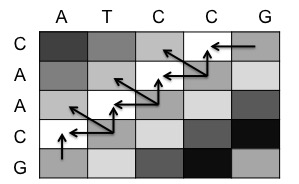
\includegraphics[width=1.8in]{Figures/Figure3C2.jpg}
		\caption {The anti-diagonal parallelism explored in the general S-W algorithm.}
		\label{fig:F3C2}
	\end{center}
\end{figure}

\subsection{S-W in BWA-MEM: An Extended S-W Algorithm} 
\label{subsec:Smith-Waterman}
In the NGS flow, a chemical sequencer chops many copies of a human genome into small segments and determines their nucleotide sequences. 
A small segment is called a read, which is generally composed of hundreds of nucleotides. 
We use the term ``base-pair'' (bp) as the unit of nucleotide. %for the rest of discussion.
Meanwhile, a pre-existing human genome is used as a reference with 3.2 billions bps \cite{Mardis2008}.
Read alignment is naturally a string matching problem. %to find the mapping between a read and the reference.
To be specific, the goal is to find a gap-tolerant mapping, i.e. an inexact mapping, between the read and the reference, that maximizes the total alignment score. 
%with a given score function that enumerates all possible character mappings.

The S-W algorithm \cite{Smith1981} is the classic approach that addresses this problem. 
This dynamic programming algorithm tolerates an arbitrary number of mismatches and gaps, 
and is guaranteed to generate the optimal solution with the highest score. 
However, the time complexity is O($nm$), which is proportional to the length of the read ($m$) and the reference ($n$). 
For the human genome, $n$ is approximately 3.2 billions, 
which makes it prohibitive for processing all the billions of reads collected from an individual using the S-W algorithm.

An alternative solution proposed in \cite{BWA} is developed based on the backward search with the Burrows-Wheeler Transform (BWT).
%which performs extremely efficiently for exact string matching. 
%Two strings are considered as exactly matched to both of them are identical. 
With the BWT-encoded reference genome, this approach achieves O($m$) time for a read to find all exactly matched substrings in the reference genome, 
independent of the size of the long reference genome. For gap-tolerant matching using backward search, 
nevertheless, the complexity is exponential.

The state-of-the-art read aligners harness both and turn to a two-step heuristic method \cite{Heng2010}. 
First, a series of substrings of a read are selected and aligned to the reference genome without gaps, i.e. exact mappings, by using BWT-based algorithms.
%This step is fast and is achieved by using BWT-based algorithms.
After that, such short un-gapped alignments serve as seeds and extended both leftward and rightward using S-W algorithm. 
Extended segments in reads are usually called queries, and their corresponding segments in the reference genome are called targets. 
This paradigm, seed-and-extend, first introduced in the famous BLAST algorithm \cite{BLAST1990}, is deemed a milestone for read alignment.
Most of the contemporary read alignment algorithms, such as SOAP \cite{SOAP}, BFAST \cite{BFAST}, LAST \cite{LAST}, Bowtie 2 \cite{Bowtie2}, and BWA-MEM \cite{BWA-MEM}, 
are derived from this canonical paradigm.

The Burrows-Wheeler Aligner (BWA) is by far the most prevalent read alignment software package \cite{BWA}\cite{BWA-SW}\cite{BWA-MEM}.
BWA-MEM \cite{BWA-MEM} is the latest generation among BWA \cite{BWA}, BWA-SW \cite{BWA-SW}, and BWA-MEM \cite{BWA-MEM}. 
BWA-MEM demonstrates better performance than several state-of-the-art tools 
and is also adaptable to a wide range of read lengths from 70bp to a few millions bps. 
The algorithm falls into the seed-and-extend category, but introduces two innovations.

First, unlike BLAST \cite{BLAST1990}, whose seed length is fixed, BWA-MEM adopts the super maximal exact matches (SMEM) method \cite{Heng2012} to generate
a group of variable-length substrings from a read as seeds; this is demonstrated in Figure \ref{fig:F1C2}. 
%a maximum exact match (MEM) is an exact string match that cannot be extended leftwards or rightwards to obtain a longer exact match, 
%and an SMEM is a MEM that is not contained in other MEMs on the read. 
An SMEM can possibly start from any location of a read and its length ranges from one to the length of a read ($m$). 
This feature results in a sharp variation of the seed lengths, which makes the sizes of inputs of the S-W algorithm vary substantially in BWA-MEM.
%BWA-MEM uses an algorithm proposed in \cite{Heng2012} to find the set of SMEMs as seeds for Smith-Waterman extension. 
%The algorithm is derived from the classic BWT-based backward search algorithm with linear time complexity, which is relatively fast compared to the quadratic Smith-Waterman extension.

\begin{figure}[!hbt]
	\begin{center}
		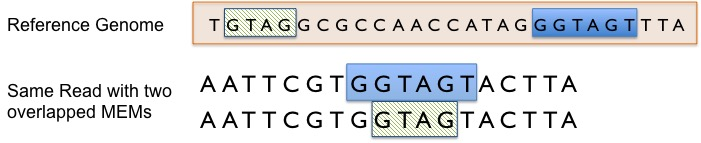
\includegraphics[width=3.2in]{Figures/Figure1C2.jpg}
		\caption {A maximal exact match (MEM) is an exact match that cannot be extended leftward or rightward without introducing a mismatch. Both of the matches illustrated are MEMs. An SMEM is a MEM that is not contained in other MEMs on the read. In this case, the longer match fully covers the shorter one on the read, and is not fully covered by any other MEM. Therefore, the longer match is an SMEM, but the shorter one is not.}
		\label{fig:F1C2}
	\end{center}
\end{figure}

%Second, as achieves the highest time complexity among all the main steps of BWA-MEM, seed extension becomes the bottleneck the whole BWA-MEM algorithm. Like other seed-and-extend algorithms, BWA-MEM adopts Smith-Waterman, a quadratic time algorithm, for seed extension. 
Second, BWA-MEM does not use the standard S-W algorithm but further extends it to improve performance. 
In general, to align two strings of length $m$ and $n$, 
a $m$x$n$ score matrix is expected to be filled up so as to generate the highest score and its corresponding alignment. 
BWA-MEM, however, developed a pruning heuristic to eliminate the solution space \cite{BWA-MEM}.
When we calculate the score at reference position $x$ and query position $y$, BWA-MEM will stop extension 
if the difference between the best extension score and the score at ($x$, $y$) is larger than $Z+\lvert x-y \rvert \times p_{gapExt}$, 
where $p_{gapExt}$ is the gap extension penalty and $Z$ is an arbitrary cutoff \cite{BWA-MEM}.
Figure \ref{fig:F2C2} illustrates the impact of the pruning strategy on a 55x105 S-W input. 
Pruning saves more than half of the computation effort than does the standard S-W algorithm. 
This pruning heuristic performs even better when reads get longer, which is the trend of further NGS \cite{Mardis2008}\cite{Heng2010}\cite{BWA-MEM}.
However, none of the existing hardware acceleration techniques can be adopted easily and efficiently to accelerate the extended S-W algorithm. 
%As is described detailedly in \cite{BWA-MEM}, the customized Smith-Waterman will stop calculating the (i+1)-th and following columns in the score matrix if the highest score in the i-th column is way lower than the highest score known so far. Inside each column, meanwhile, only part of the score matrix elements are actually filled due to the existence of the pruning strategy. Figure \ref{fig:F2C2} illustrates the impact of the pruning strategy on a 55x105 score matrix. The two strings for alignment are 55bp and 105bp long respectively, and the standard Smith-Waterman algorithm should fill up a matrix with 5775 elements. Actually, only 2836 elements got calculated which means more than 50\% of the elements are pruned out in the BWA-MEM Smith-Waterman, meaning 2x speedup achieved.

\begin{figure}[!hbt]
	\begin{center}
		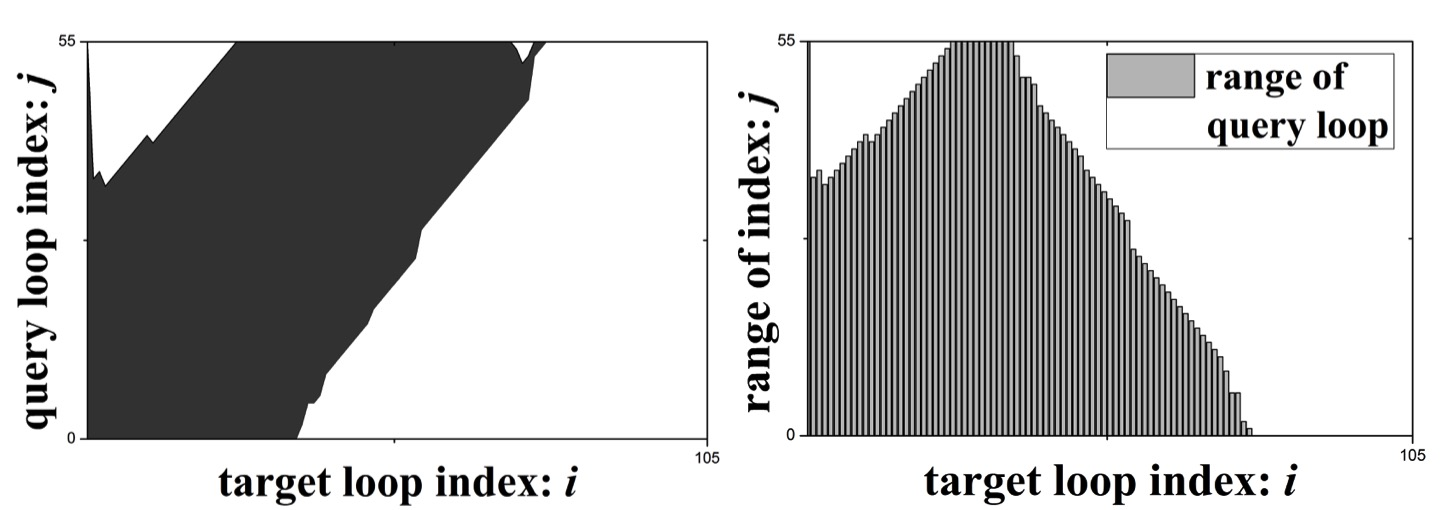
\includegraphics[width=3.2in]{Figures/Figure2C2.jpg}
		\caption {A 55x105 BWA-MEM Smith-Waterman task. The general S-W algorithm requires filling up a 55x105 matrix (5775 elements), but only 2836 elements (49\%) were actually filled with the help of pruning. The shaded area in the left graph illustrates the elements that got filled, and the right graph shows how many elements for each target loop index are actually calculated.}
		\label{fig:F2C2}
	\end{center}
\end{figure}

%The inefficiency of the wavefront-based technique will be discussed in the next section.

%\subsection{Inefficiencies of the Wavefront Technique in BWA-MEM} 
%\label{subsec:inefficiency}

%As a fundamental operation in computational genetics, the S-W algorithm has attracted a large amount attention from academia \cite{Aluru2014}. 
%The general S-W algorithm is inherently anti-diagonal parallelizable, 
%since the elements along each anti-diagonal in the S-W matrix are independent of each other, 
%and each element only depends on three elements from the previous two anti-diagonals \cite{Edmiston1988}. 
%Therefore, the wavefront property, as illustrated in Figure \ref{fig:F3C2}, 
%has been used by researchers in almost all kinds of platforms for the S-W algorithm acceleration \cite{Wozniak1997}\cite{Arram2013}\cite{Preusser2012}\cite{Olson2012}\cite{RaceLogic}.
%\begin{figure}[!hbt]
%	\begin{center}
%		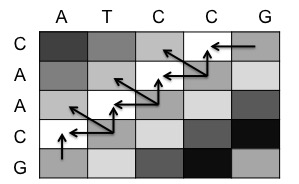
\includegraphics[width=1.8in]{Figures/Figure3C2.jpg}
%		\caption {Inherent anti-diagonal parallelism explored in S-W algorithm.}
%		\label{fig:F3C2}
%	\end{center}
%\end{figure}

%Nevertheless, tools such as BLAST \cite{BLAST1990} and BWA-MEM \cite{BWA-MEM} use the customized versions of the S-W algorithms.
%In BWA-MEM, we have three important observations that prevent us from using conventional wavefront technique for hardware acceleration.
%For simplicity of without lossing generality, 
%we abstract an acceleration platform to into a given number of unified processing elements (PEs) in the following discussions. 
%Each PE in the platform is capable to produce one DP computation per cycle to fill the score matrix. 
%A \textit{kernel} is composed of a group of PEs and can be assigned to execute one S-W task.
%We denote $m$x$n$ as a pair of input strings for S-W algorithm with length $m$ and $n$, respectively. 
%The maximum achievable degree of parallelism is bounded by the length of the shorter string.



\section{Basis of Our Approach}
\label{sec:approach}

%Nevertheless, tools such as BLAST \cite{BLAST1990} and BWA-MEM \cite{BWA-MEM} use the customized versions of the S-W algorithms.
%In BWA-MEM, we have three important observations that prevent us from using conventional wavefront technique for hardware acceleration.
Our acceleration engine design is based on the following three important observations 
derived from an analysis of the S-W implementation in BWA-MEM.
%%%From the observations, we find that the wavefront-based architectures are inefficient to be applied in BWA-MEM.
%%%
For simplicity without losing generality, 
we abstract the total resources of an accelerator platform into a given number of unified processing elements (PEs). 
We also assume that each PE is capable of producing one value per cycle to fill the 2D table in the DP algorithm. 
A \textit{kernel} is composed of a group of PEs and can be assigned to execute one S-W task.
We denote $m$x$n$ as a pair of input strings for the S-W algorithm with length $m$ and $n$. 
%%%The maximum achievable degree of parallelism is bounded by the length of the shorter string.

\vspace{1pt}
\textbf{Observation 1: Enormous Task-Level Parallelism}
\vspace{1pt}

A sequencer can generate billions of reads from a single individual for analysis in today's NGS flow.
The huge amount of data generates enormous task-level parallelism, prompting us to reexamine the conventional wavefront technique for S-W acceleration.
The conventional wavefront technique exploits the inner-task anti-diagonal parallelism to maximize the speedup for a single task.
However, the wavefront implementation is not optimal when the task-level parallelism is several orders of magnitude larger than the inner-task parallelism.
%%%This is because the resources for implementing accelerators is limited.
For an accelerator platform with limited resources provided, e.g., a FPGA board with a certain amount of LUTs (DSPs, BRAMs, etc.), we must decide if the resources should be allocated for exploiting the task-level parallelism or the inner-task parallelism.

%%%The three designs listed in Table \ref{tab:example} are used to demonstrate the performance impact on low PE utilization.
%%%We use 40 12x50 S-W tasks as input.
%%%Both Design 1 and Design 2 use the wavefront technique, which has multiple PEs in one kernel, 
%%%in order to exploit the inner-task parallelism.
%%%Design 3 has the maximum number of kernels and can fully exploit the task-level parallelism.
%%%With the same number of PEs, Design 3 outperforms the others since its PEs are fully utilized all the time.
%%%For Design 1, the maximum degree parallelism is 12, which is not divisible by the number of PEs per kernel (8).
%%%Therefore, some of the PEs are not fully utilized and it leads to poor performance.
%%%
%%%\input TBL/example
%%%
\vspace{1pt}
\textbf{Observation 2: Significantly Varied-Size Inputs}
\vspace{1pt}

The sharply varied input sizes of S-W in BWA-MEM result in a considerable waste of resources in wavefront-based designs. 
For example, a kernel of 10 PEs is only able to reach at most a 65\% resource utilization for a 13x103 input because the length of the maximal anti-diagonals (13) is not divisible by the number of PEs (10). It takes 2 cycles for 10 PEs in filling an anti-diagonal with 13 elements.
Figure \ref{fig:F4C2} provides a histogram of the sizes of the shorter strings (bounding the maximum degrees of parallelism) over 10M inputs of randomly selected BWA-MEM S-W tasks. 
The sizes range from one to 84, and none of them has more than 5\% of the 10M inputs. 
The significant diversity of input sizes makes it prohibitive to choose one or a few kinds of PEs to avoid wasting resources.
A better choice is to have each kernel restricted to only one PE, which means the anti-diagonal parallelism gets totally ignored.
%Assume that there is a kernel of 10 PEs to execute a 10x30 Smith-Waterman task. A 10x30 matrix has 39 anti-diagonal, each of which has at most 10 elements, so it takes 39 cycles for our 10-PE kernel to finish the task. However, the 10 PEs get fully utilized in only 21 cycles and the total PE utilization ratio is only 77\%, because of the filling and draining of the pipeline. The filling and draining inefficiency can be ignored if the input size is relatively large compared to the kernel size, e.g. a 10x10,000 task on a 10-PE kernel, but the inputs of BWA-MEM Smith-Waterman do not fall into this category. Figure \ref{fig:F4C2} provides a histogram of the lengths of the shorter strings (bounding the maximum degrees of parallelism) over 10 million randomly selected BWA-MEM Smith-Waterman tasks. The average length of the shorter strings is only 34 and approximately 25\% of the inputs has their shorter strings less than 10 in length. Configuring each kernel in a large size will surely lead to a low resource utilization rate in BWA-MEM.
%Another source of inadequate utilization comes from the irregular sizes of inputs. For a kernel of 10 PEs fed by a 13x37 Smith-Waterman task, the 13-element anti-diagonal has to consume 2 cycles, and the second cycle calculates only 3 elements, leaving 7 PEs unused and 65\% utilization rate in the two cycles. Admittedly, it has potential for the 10 PEs to calculate elements crossing anti-diagonals, but the control logic of each PE will consequently become much more complicated and take more area, which in turn decrease the number of PEs an accelerator platform can form. Based on our profiling over 10 million randomly selected tasks, the length of the shorter string ranges from 1 up to 84 consecutively, without any number showing up more than 5\%. Therefore, this kind of inefficient utilization is inevitable in BWA-MEM unless each kernel has only 1 PE.

\vspace{1pt}
\textbf{Observation 3: Pruning Strategies}
\vspace{1pt}

Derived from the X-dropoff pruning strategy in BLAST \cite{BLAST1990}, 
BWA-MEM's pruning strategy is able to save over 50\% in computation efforts for S-W tasks, as illustrated in Figure \ref{fig:F2C2}. 
%%%BWA-MEM's pruning strategy is able to save over 50\% in computation efforts for S-W tasks, as discussed in Section \ref{subsec:Smith-Waterman}. 
However, the pruning strategy destroys the basis of the anti-diagonal parallelism, as described in detail in \cite{BWA-MEM}. 
Moreover, the results generated by the optimized S-W algorithm in BWA-MEM will be slightly different from those obtained by the standard S-W algorithm. 
This increases the difficulty of integrating existing wavefront-based work into BWA-MEM. 
Even if the difficulty of integration can be overcome, 
the potential speedup from pruning would have to be sacrificed due to its incompatibility with the wavefront technique.
It will be even worse when the sizes of seeds become longer, which is the future trend for NGS.
%%%For Design 3 illustrated in Table \ref{tab:example}, it can be further accelerated by 2x with 50\% of computation pruned (1500 cycles). 
%%%However, the wavefront-based architectures, like Design 1 and 2, cannot leverage the benefits of pruning.

\begin{figure}[!hbt]
	\begin{center}
		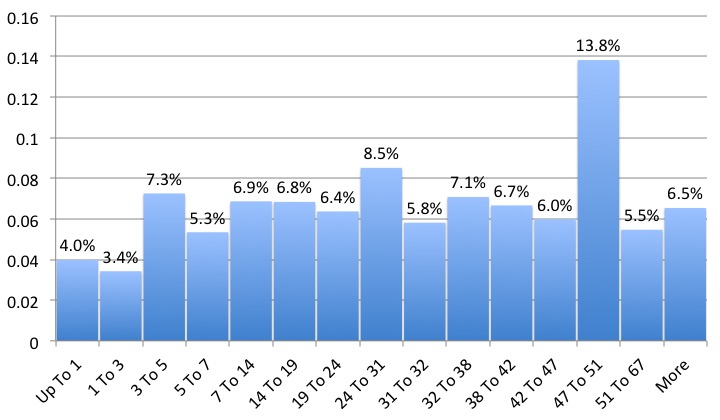
\includegraphics[width=2.5in]{Figures/Figure4C2.jpg}
		\caption {Histogram of the lengths of the shorter input strings collected from 10 million randomly selected BWA-MEM S-W tasks.}
		\label{fig:F4C2}
	\end{center}
\end{figure}
\vspace{-15pt}

\begin{figure}[!hbt]
	\begin{center}
		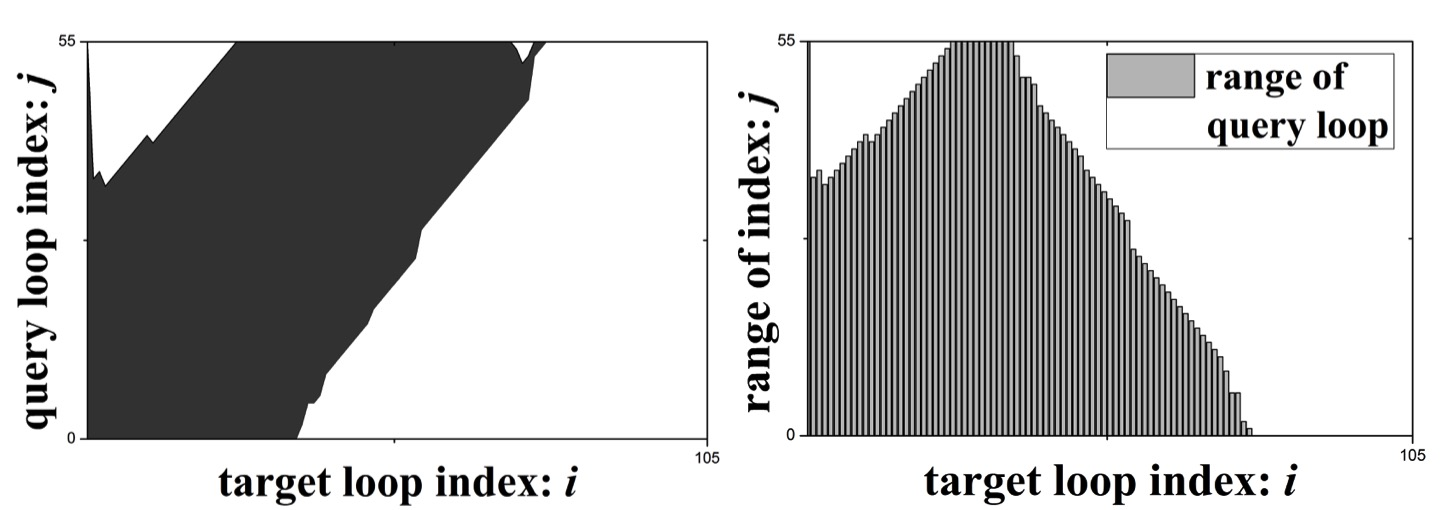
\includegraphics[width=2.5in]{Figures/Figure2C2.jpg}
		\caption {A 55x105 BWA-MEM Smith-Waterman task. The general S-W algorithm requires filling up a 55x105 matrix (5775 elements), but only 2836 elements (49\%) were actually filled with the help of pruning. The shaded area in the left graph illustrates the elements that got filled, and the right graph shows how many elements for each target loop index are actually calculated.}
		\label{fig:F2C2}
	\end{center}
\end{figure}
\vspace{-10pt}

%%%%\subsection{Simple is Best: A Motivational Example} 
%%%%\label{subsec:motivation}
%%%
%%%%The three key observations described in Section \ref{subsec:inefficiency} inspire us to develop a novel architecture 
%%%%for the customized S-W algorithm to replace the traditional wavefront-based design. 
%%%%Before we discuss the details of the architecture design, a motivational example is used to illustrate the inefficiency of wavefront technique.
%%%%We assume that a given accelerator platform has eight PEs in total based on the resource constraint and is fed with 40 12x50 Smith-Waterman tasks. 
%%%%We compare three design choices listed below.
%%%
%%%%\vspace{1pt}
%%%%\textit{Design 1: 1 kernel of 8 PEs}
%%%
%%%%\vspace{1pt}
%%%%\textit{Design 2: 2 kernels, 4 PEs per kernel}
%%%
%%%%\vspace{1pt}
%%%%\textit{Design 3: 8 kernels, 1 PE kernel}
%%%%\vspace{1pt}
%%%
%%%%Design 1 assigned all the resources to a single kernel and thus this kernel is the fastest kernel among all designs. 
%%%%However, since the maximum degree of parallelism ($12$) is not divisible by the kernel size ($8$), some of the PEs are idled during computation. 
%%%%The latency of each task and the total execution time is 106 and 4240 cycles, respectively.
%%%
%%%%For Design 2, the PEs are almost fully utilized since the maximum degree of parallelism ($12$) is divisible by the kernel size ($4$). 
%%%%The latency of each task and the total execution time is 159 and 3180 cycles, respectively.
%%%
%%%%Design 3 reaches the other extreme by abandoning anti-diagonal parallelism. 
%%%%Each kernel has the longest latency, 600 cycles, among all three designs. 
%%%%However, Design 3 can achieve the maximum degree of task-level parallelism, and thus achieves the ideal 3000-cycle runtime.
%%%
%%%%This example clearly demonstrates the design scheme that maximizes the number of simple kernels can lead to better performance
%%%%when the task-level parallelism dominates.
%%%%A wavefront-based kernel with multiple PEs reduces the latency of a task, but at the cost of low resource utilization. 
%%%%It only works well when 1) the task-level parallelism is limited, or 2) the input size is homogeneous. 
%%%
%%%%However, for BWA-MEM, the task-level parallelism is almost infinite as pointed out in Observation 1.
%%%%Also, the input sizes of S-W tasks vary sharply as discussed in Observation 2. 
%%%%In this case, the throughput becomes vital and the latency improvement by exploiting the inner-task parallelism is limited. 
%%%%That is why Design 3 outperforms the others since each PE can be fully utilized all the time.
%%%
%%%%Furthermore, while Design 2 can also achieve great resource utilization rate, 
%%%%Design 3 still works better since the pruning heuristic (Observation 3) can be integrated into the accelerator design. 
%%%%Design 3 gives the flexibility to calculate one element in the score matrix per cycle in any arbitrary order, 
%%%%rather than only follows the anti-diagonal pattern.
%%%%This makes Design 3 easily adapt to the pruning strategy in BWA-MEM.
%%%%Presuming that half of the score matrix elements can be pruned, 
%%%%Design 3 shows the potential to reach 300 cycles per task and 1500 cycles in total, i.e. extra 2x speedup.
%%%%We also have to mention that the score matrix filling order in BWA-MEM is column by column, 
%%%%which further prevents the integration with the wavefront technique used the anti-diagonal execution order.
%%%
%%%
%%%%\subsection{From Ideal to Reality: Challenges to Face} 
%%%%\label{subsec:challenges}
%%%%
%%%%The motivation example points out the principle of our design: abandoning wavefront, fully utilizing pruning and pursuing task-level parallelism. This principle is not merely fitted into BWA-MEM, but probably suitable for most of the scale-out applications. With the advent of the “big-data” era, scale-out applications, conceiving drastic task-level parallelism, draw more and more attention. Task throughput instead of latency is essential for the performances of these applications. For an accelerator platform with limited resources, the resource utilization rate of design becomes a critical parameter.
%%%%
%%%%For Smith-Waterman, the wavefront technique is inherently unable to 100\% utilize all the resources due to the filling and draining of the pipeline. Random sizes of inputs deteriorate the situation, because no matter how many PEs assigned to a kernel, at least 50\% of the inputs are indivisible by the size of the kernel, unless one kernel allocates only one PE. Worse still, wavefront is contradictory to the pruning strategy, which leads to approximately half of the computation effort is actually unnecessary. A 1-PE kernel has potential to eliminate these problems effectively. There is not any filling and draining overhead, and indivisibility problem for a 1-PE kernel. Moreover, 1-PE kernel, which is independent of anti-diagonal parallelism, is likely to fit into all kinds of pruning strategies, which in turn boost the performance of the design.
%%%%
%%%%To turn the potential to an actual speedup, however, two challenges have to be fought off.
%%%%
%%%%\vspace{1pt}
%%%%\textbf{Challenge 1: Reduce the overhead of pruning}
%%%%\vspace{1pt}
%%%%
%%%%In BWA-MEM, the pruning process will occur when one column of the score matrix finishes calculation. Then, the maximal score in this column and the maximal score known so far will be checked with some dynamically changed threshold to determine the left bound and right bound of the next column. After the pruning, only the elements between the decided left and right bound in the next column will be calculated. Apparently, this complicated logic will suspend the calculation of matrix elements, leading to performance degradation.
%%%%
%%%%\vspace{1pt}
%%%%\textbf{Challenge 2: Reduce the overhead of task scheduling}
%%%%\vspace{1pt}
%%%%
%%%%Similarly with multi-core/many-core architectures in the CPU design area, a large amount of kernels lead to complicated scheduling. Without any optimization, the scheduling logic will take a considerable amount of resources and sometimes become dominant since the kernel is supposed to be simplified to have only 1 PE.
%%%%
%%%%The next chapter will describe our PE architecture and scheduling strategy, and propose our solutions against the two challenges.

\section{ARCHITECTURE DESIGN AND IMPLEMENTATION} 
\label{sec:architecture}
\subsection{Overall Architecture}

Our accelerator engine consists of multiple PE arrays connecting with the off-chip memory via AXI bus interface, as shown in Figure \ref{fig:overall_architecture}.
Each PE acts as one kernel and can take one S-W task to maximize throughput.

\begin{figure}[!hbt]
\begin{center}
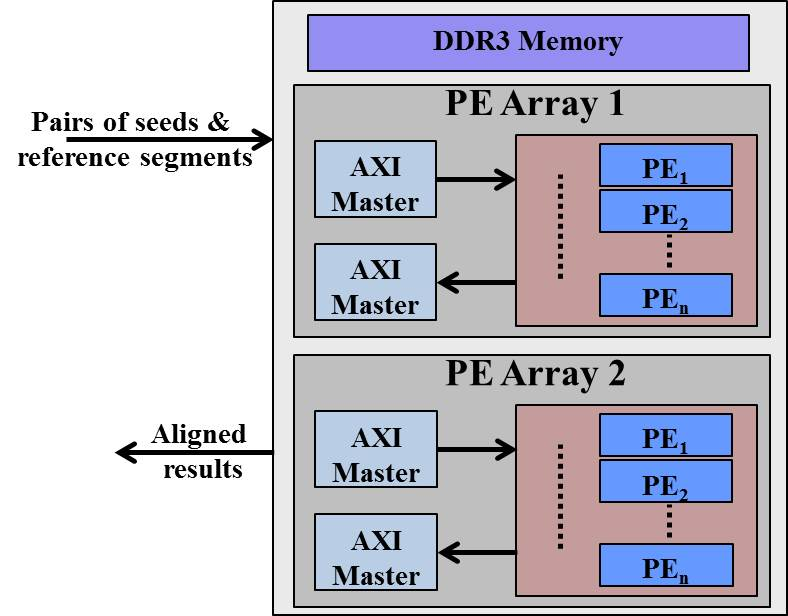
\includegraphics[width=2.8in]{Figures/Figure_Arch1.jpg}
\caption {Overall architecture of the proposed accelerator engine} \label{fig:overall_architecture} \end{center} \end{figure}

Before the accelerator starts to operate, the host processor assembles a set of query and target sequence pairs and streams them to the on-board DDR3 memory via PCIe. 
Then, each PE array's task distributor fetches a certain part of sequence pairs and distributes them to the idled PEs. 
The resulting mappings are stored in the on-board memory and then sent back to the host.

\subsection{Processing Element (PE) Design}

A PE realizes the S-W code obtained from the software implementation in BWA-MEM. 
We design our PE architecture using the high-level synthesis methodology. 
Unlike wavefront-based solutions which looks completely different from the software approach,  
our design natrually follows the original software approach, which considerably shortens the development period. 

To maximize throughput, we make the initiation interval (II) be equal to 1 (II=1), i.e. calculating one cell of the score matrix per cycle. 
Moreover, a piece of conditional branch logic is implemented to realize pruning. 
It enlarges the size of each PE by 20\%, but reduces computation effort by over 50\%.  
%%%To maximize the throughput, we have to make the initiation interval (II) of the inner loop be equal to 1 (II=1). 
%%%To achieve ``II=1'', we propose the following microachitecture improvements. 
%%%First, we merge \textit{loop\_bounds\_update()} into the inner loop so that the update of \emph{beg} and \emph{end} 
%%%can be done in parallel with \textit{score\_calculation()}.
%%%Second, both the read and write operations of array \emph{e} and \emph{h} occur at the same cycle.
%%%The proposed solution is to realize the two arrays by using dual-port BRAM blocks
%%%and insert registers to guarantee that the read and write addresses are different.
%%%Listing \ref{list:ksw_extend2} shows the C kernel function, \textit{ksw\_extend2()}, 
%%%which contains a two-level nested loop to accomplish the alignment procedure.
%%%The two sequence arrays, \textit{query} and \textit{target}, are sent to the function as inputs.
%%%The other inputs are constants (\emph{o\_del}, \emph{e\_del}, \emph{o\_ins}, and \emph{e\_ins}) or the outputs from previous host functions (\emph{h0}).
%%%Array \emph{e} and \emph{h} are used to keep temporary scores.
%%%From a high-level point of view, the function is composed of four subfunctions: 
%%%(1) \textit{init()}, (2) \textit{score\_calculation()}, (3) \textit{loop\_bounds\_update()}, and (4) \textit{results\_generation()}.
%%%\textit{score\_calculation()} can fill one element in the score matrix
%%%while \textit{loop\_bounds\_update()} calculates the beginning point (\emph{beg}) and the ending point (\emph{end}) for the next iteration for pruning.
%%%
%%%
%%%%Figure \ref{fig:pe_archi} shows the architecture design of a PE.
%%%%The \emph{query} and \emph{target} arrays store the sequences of the input seed and the reference genome segment.
%%%%In the outer loop, the kernel traverses the \emph{target} array, where \emph{i} is the array index.
%%%%In the inner loop, the kernel traverses the \emph{query} array (index: \emph{j}) and fills all the elements successively in this column in the score matrix. 
%%%%A table lookup in the \textit{match table} is required to compute a temporary value (\emph{t}) for the current element. 
%%%%Moreover, the kernels also need to look up two more scores from the up-left and left neighbors, which have been computed in the previous outer-loop iteration.
%%%%These two scores of the two neighbors are saved in \emph{h}[\emph{j}] and \emph{e}[\emph{j}], respectively.
%%%%The score of the up neighbor is stored in register \emph{f}.
%%%%With \emph{t}, \emph{f}, \emph{h}[\emph{j}] and \emph{e}[\emph{j}], the score of the current position can be computed.
%%%
%%%We design our PE architecture by using the high-level synthesis methodology \cite{Cong2004}.
%%%Figure \ref{fig:pe_archi} shows the architecture design of a PE.
%%%To maximize the throughput, we have to make the initiation interval (II) of the inner loop be equal to 1 (II=1). 
%%%To achieve ``II=1'', we propose the following microachitecture improvements. 
%%%First, we merge \textit{loop\_bounds\_update()} into the inner loop so that the update of \emph{beg} and \emph{end} 
%%%can be done in parallel with \textit{score\_calculation()}.
%%%Second, both the read and write operations of array \emph{e} and \emph{h} occur at the same cycle.
%%%The proposed solution is to realize the two arrays by using dual-port BRAM blocks
%%%and insert registers to guarantee that the read and write addresses are different.
%%%
%%%\begin{lstlisting}[language={c++},basicstyle=\small,
%%%caption={The ksw\_extend2() in BWA-MEM: a high-level view.},
%%%captionpos=b,
%%%label={list:ksw_extend2}]
%%%void ksw_extend2(int qlen, uint8_t *query, 
%%%   int tlen, uint8_t *target, int o_del, 
%%%   int e_del, int o_ins, int e_ins, int h0, 
%%%   ...)
%%%{
%%%   ...
%%%
%%%   // outer loop
%%%   for(int i = 0; i < tlen; i++) {
%%%      init();
%%%      // inner loop
%%%      for(int j = beg; j < end; j++) {
%%%         // fill one element in score matrix
%%%         score_calculation(query[j],
%%%            o_del, e_del, o_ins, e_ins, 
%%%            h0, e, h, i, j, ...);
%%%      }
%%%      // perform pruning
%%%      loop_bounds_update(mj, h, &beg, &end);
%%%      results_generation(mj, m);
%%%   }
%%%   ..
%%%}
%%%\end{lstlisting}
%%%
%%%\begin{figure}[!hbt]
%%%\begin{center}
%%%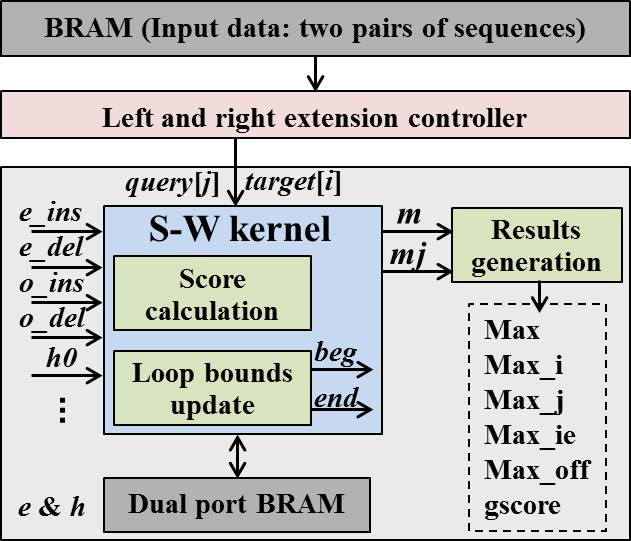
\includegraphics[width=2.8in]{Figures/Figure_Arch3.jpg}
%%%\caption {Architecture Design of a PE} \label{fig:pe_archi} \end{center} \end{figure}
%%%
%%%%First, the operation of reading BRAM data and the lookup in the \textit{match table} must complete in one clock cycle. 
%%%%Therefore, the \textit{match table} is implemented as individual registers. 
%%%%Second, both the read and write operations of array \emph{h} and \emph{e} occur at the same cycle. 
%%%%The proposed solution is to realize the two arrays by using dual-port BRAM blocks 
%%%%and insert registers to guarantee that the read and write addresses are different.
%%%
%%%Furthermore, since the extensions need to be performed in both ends of a seed,
%%%we merge both the left and right extention capability into our PE design and reuse the same S-W kernel, 
%%%as shown in Figure \ref{fig:pe_archi}.

\subsection{Two-level Task Scheduling}

\begin{figure}[!hbt]
\begin{center}
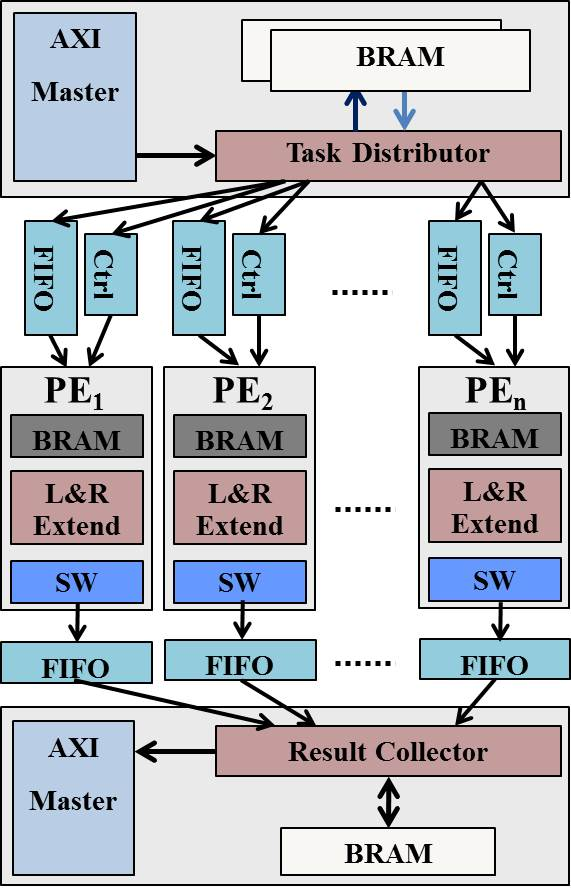
\includegraphics[width=2.4in]{Figures/Figure_Arch2.jpg}
\caption {The design of a PE array} \label{fig:schedule_structure} \end{center} \end{figure}

The first-level of task scheduling resides in a PE array. 
A PE array includes three types of major components: (1) \textit{task distributor} (2) \textit{PE}, and (3) \textit{result collector}, 
as shown in Figure \ref{fig:schedule_structure}.
The \textit{task distributor} fetches data from the on-board DRAM to the on-chip BRAM and dynamically dispatches the tasks to each PE through a FIFO.
%%%A PE array contains a number of PEs to read data from their own FIFOs and process the S-W tasks in parallel.
The \textit{result collector} receives mapping results from each PE through a FIFO and packs them together for the host.

If a centralized \textit{task distributor} is not provided, each PE needs to fetch data from on-board memory independently. 
This incurs a significant (25\%) area overhead per PE to synthesize its own AXI interface. 
To reduce the overhead, we use only one AXI bus master for each \textit{task distributor} per PE array. 
The bus master fetches a group of data each time that meets the off-chip bandwidth demand of all PEs in the array. 
We also implement the ping-pong buffer operation by using double BRAM blocks for better performance. 
After the data are prefetched to BRAM, 
the distributor will check the flag of the FIFO of each PE (marked as $Ctrl$ in Figure \ref{fig:schedule_structure}) one by one to find out the available PEs. 
The \textit{task distributor} then transfers the S-W tasks from BRAM to the FIFOs of the available PEs. 
This process continues until all the tasks are processed.
The \textit{result collector} keeps monitoring the output FIFO of each PE and obtaining results until all the results are received.

If the number of PEs is small, the first-level of task scheduling is capable enough. 
However, when the number of PEs is increased to a certain point, 
the distributor becomes a performance bottleneck caused by its round-robin task scheduling manner.
Therefore, we explore the second-level of task scheduling by replicating the nubmer of PE arrays, i.e. the number of \textit{task distributors}. 
This two-level hierarchy provides us with a design methodology for obtaining scalable speedup with more PE arrays.


%\subsection{High-level Synthesis Implementation}

%All the above mentioned structures are described in C code and translated into RTL verilog code by the Vivado HLS tool. In addition, we take advantage of some special definitions and directives to guide the HLS tool to create the expected hardware architecture. For instance, the variable type of HLS stream is used to connect the three main parts with FIFOs (\ref{fig:pe_archi}). And the dataflow directive is utilized to make the parts run in parallel.

%Derived from the benefit of high-level synthesis technique, the proposed architecture is easy to be adjusted for achieving scalability of acceleration, only by modifying a couple of parameters which define the number of duplication.



\section{Experimental Results} 
\label{sec:results}
\subsection{Experimental Setup}
Our design is described in HLS C and synthesized using Vivado HLS.
The accelerator engine contains two PE arrays, each of which is composed of 50 PEs, and can run at 150MHz on the Xilinx VC707 FPGA evaluation board.
The FPGA resource utilization is approximately 65\% (LUT: 65.4\%, Reg: 30.7\%, etc.). 
We use an input with 100M of reads, which is a subset collected from a real individual human genome sample (about 500M reads, 120GB FASTQ file) with breast cancer (HCC1954). 
We verify the outputs of our FPGA implementation with the seed extension step of BWA-MEM to ensure correctness. 
\subsection{Speedup over Software-Based BWA-MEM}
To demonstrate the speedup of our accelerator engine over the original BWA-MEM software, 
an Intel Haswell Xeon server loaded with two 6-core CPUs is used.
The server has 24 threads in total with hyperthreading support.
We compare the execution time of our FPGA implementation with pure software customized S-W runtimes with 1, 2, 4, 8, 16 and 24 threads, respectively.
To make it a fair comparison, only the computation time of the S-W calls (after loading inputs from memory and before storing outputs to memory) is collected for both FPGA and CPU implementations.

Figure \ref{fig:F1C5} shows the performance comparison between our FPGA design and the original BWA-MEM software with results normalized to the single-threaded CPU performance.
Our FPGA design outperforms the 24-thread CPU by 26.4 times.
\begin{figure}[!hbt]
	\begin{center}
		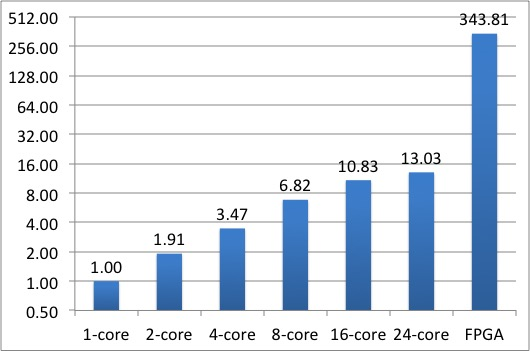
\includegraphics[width=2.5in]{Figures/F1C5.jpg}
		\caption {Performance comparison between the FPGA design and the multi-threaded software BWA-MEM.}
		\label{fig:F1C5}
	\end{center}
\end{figure}
\subsection{Speedup Over Wavefront-Based Designs}
To highlight the advantage of our design over wavefront-based solutions, 
we compare the runtime of our accelerator engine to those of a set of wavefront-based FPGA implementations described in \cite{Zhang2007}, in which a circuit-level design is delivered. To have a fair comparison, we try to implement all designs with roughly the same FPGA resource utilization.

Table \ref{tab:configuration} shows the wavefront-based designs we created for comparison. 
A design containing $n$ kernels with $m$ PE per kenel is denoted by $m$Px$n$K. 
We use a 32Px5K configuration, which is the slowest among all FPGA designs, as the base unit for comparison.
We find that the performance of the wavefront-based designs generally decreases when the number of PE per kernel ($m$) increases.
although the performance does not decrease fully monotonically, as shown in Figure \ref{fig:F2C5}.
In general, this shows that the wavefront-based designs have worse PE utilization rates compared to our design. 

Furthermore, Figure \ref{fig:F2C5} also demonstrates the power of pruning. 
When the wavefront design comes to one extreme with only one PE per kernel (1Px116K), 
the only difference between our design and the 1Px116K design is whether the pruning logics are realized. 
Compared to the 1Px116K design, our design shows about 2x speedup.
%%% even though the number of PEs in our design is only 100, which is 16 PEs fewer than that of 1Px116K. 
Our current design uses the reads with length of 101bp.
Since the trend of NGS will generate longer reads in the future, the performance improvement lead by pruning is expected to be much more significant.
%%%
%%%We need to mention that resources can be saved when more PEs are integrated into one kernel for the wavefront-based designs.
%%%First, the PEs in one kernel can share one copy of control logics. A design with a large number of kernels spends more resources on the control logics.
%%%Moreover, for the wavefront implementations, the logics for pruning are not required.
%%%That is why the 32Px5K design can contain 60\% more PEs than that of our design.

\input TBL/resource_alloc

%%%\subsection{The Effectiveness of Pruning}
\begin{figure}[!hbt]
	\begin{center}
		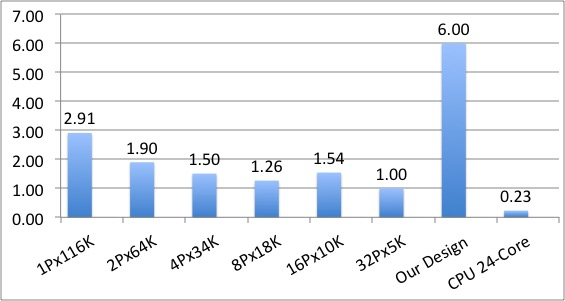
\includegraphics[width=2.5in]{Figures/F2C5.jpg}
		\caption {Performance comparison between our design and a set of wavefront-based designs.}
		\label{fig:F2C5}
	\end{center}
\end{figure}
%%%\subsection{The Need for Two-Level Scheduling}
%%%
%%%%We find that the efficiency of the task distributor can potentially become the performance bottleneck 
%%%%since the sequential round-robin scheduling becomes the critical path when the number of PEs in a PE array increases.
%%%%Compared to our accelerator engine with two PE arrays, the performance of the single PE array design is 38.9\% worse.
%%%%Both of them have 100 PEs in total.
%%%
%%%The efficiency of the task distributor can potentially become the performance bottleneck.
%%%Figure \ref{fig:F3C5} shows the performance of a PE array with different numbers of PEs.
%%%Before the number of PEs in a PE array reaches a threshold,
%%%the performance can scale almost linearly proportional to the number of PEs.
%%%The performance of a PE array scales poorly when the number of PEs is larger than 50 in our design.
%%%Therefore, to optimize system performance, our accelerator engine uses two-level scheduling and thus has two PE arrays. 
%%%Each PE array contains 50 PEs. The FPGA resource constraint prevents us from adding more PE arrays.
%%%
%%%\begin{figure}[!hbt]
%%%	\begin{center}
%%%		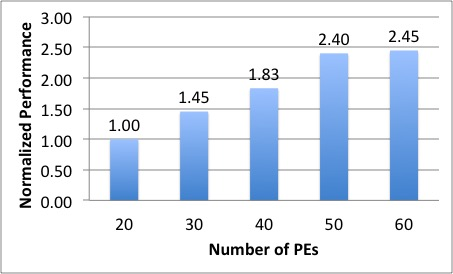
\includegraphics[width=2.8in]{Figures/F3C5.jpg}
%%%		\caption {The performance scalibility of a PE array with different numbers of PEs.}
%%%		\label{fig:F3C5}
%%%	\end{center}
%%%\end{figure}

%%%\section{Related Work} 
\label{sec:related_work}
%%%As a fundamental operation in computational biology, aligning two sequences has attracted much attention \cite{Aluru2014}. 
%%%Two classic dynamic programming algorithms, Needleman-Wunsch \cite{Needleman1970} and Smith-Waterman \cite{Smith1981}, 
%%%are proposed for global and local alignments, respectively. 
%%%Although both of them are gap/mismatch-tolerant and optimal, 
%%%the quadratic time complexity prohibits them from some real applications such as DNA sequencing. 
%%%A pure S-W based aligner is currently used as a golden reference for accuracy evaluation of alignment algorithms \cite{Bowtie2}\cite{Knodel2011}.
%%%
%%%BWT-based software aligners, such as BWA \cite{BWA} and Bowtie \cite{Bowtie}, 
%%%are dominating in the genomics area and turning into the de facto standard. 
%%%BWT-based backward search is incredibly fast for exact matching, but exponential for mismatch/gap-tolerant matching. 
%%%Therefore, the state-of-the-art alignment algorithms usually combine both the backward searching and S-W algorithm 
%%%to perform the seeding step (exact mapping), and gap/mismatch-tolerant extension step (inexact mapping), respectively \cite{Heng2010}.
%%%
%%%Different seed-and-extend algorithms accentuate different steps. 
%%%Some algorithms, such as BFAST \cite{BFAST}, perform extension only when there is no exact match found for a read. 
%%%Since the majority of the reads are able to find at least one exact match, the computation bottleneck is the seeding step. 
%%%The other algorithms, such as BWA-MEM \cite{BWA-MEM}, do left/right extensions using customized S-W algorithms for almost all reads. 
%%%Some reads can generate a large number of seeds, like 8000, for seed extension. 
%%%Therefore, the extension step becomes the bottleneck.
%%%
%%%Hardware acceleration for read alignment have been studied on all major accelerator platforms \cite{Aluru2014}\cite{Fernandez2010}. 
%%%A few studies have been proposed for BWT-based aligners,
%%%such as BWA and BFAST \cite{Arram2013}\cite{Olson2012}\cite{Wayne2013}. 
%%%However, these studies \cite{Arram2013}\cite{Olson2012}\cite{Wayne2013} focus on accelerating the backward search step, 
%%%which is different from our focus on accelerating the customized S-W algorithms.
The anti-diagonal parallelism has been explored and implemented in different ways on different platforms for S-W acceleration \cite{Preusser2012}\cite{RaceLogic}\cite{Zhang2007}\cite{Kim2011}\cite{Lam2013}. 
%%%The SIMD implementations in X86 processors take the column-based methodology for acceleration \cite{Farrar2007}\cite{Rognes2011}.
It works fairly well when the inputs are homogeneous. 
Nevertheless, contemporary read aligners such as BWA-MEM, Bowtie 2 and LAST, generate S-W inputs with highly varied sizes. 
Simply reusing the well-developed wavefront-based technique in the previous work does not work efficiently, as discussed in this paper.

Software-based pruning strategies have been realized in many software aligners, such as BLAST \cite{BLAST1990}, LAST \cite{LAST} and BWA-MEM \cite{BWA-MEM}, and are ignored in previous work. In this paper, we investigate on how to integrate the pruning strategies into the accelerator design.

\section{Conclusions} 
\label{sec:conclusions}
In this paper, we design an architecture to efficiently accelerate S-W, the computation bottleneck in BWA-MEM, the state-of-the-art read aligner. 
Massive task-level parallelism, sharply varied input sizes and software pruning strategies are emphasized in our design. 
Our FPGA implementation demonstrates about 26.4x speedup compared to a 24-thread Intel Xeon server, as well as up to 6x over wavefront-based implementations. 

\begin{figure}[!hbt]
	\begin{center}
		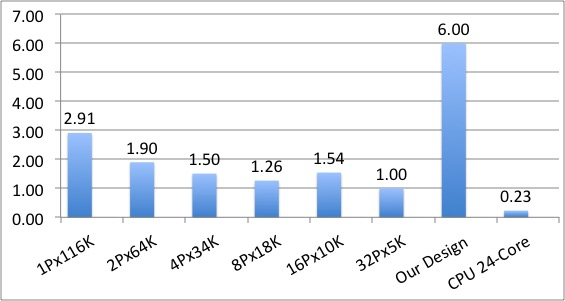
\includegraphics[width=2.5in]{Figures/F2C5.jpg}
		\caption {Performance comparison between our design and a set of wavefront-based designs.}
		\label{fig:F2C5}
	\end{center}
\end{figure}
\vspace{-10pt}


%%%\section{Introduction}
%%%% no \IEEEPARstart
%%%This demo file is intended to serve as a ``starter file''
%%%for IEEE conference papers produced under \LaTeX\ using
%%%IEEEtran.cls version 1.7 and later.
%%%
%%%All manuscripts must be in English. These guidelines include complete descriptions of the fonts, spacing, and related information for producing your proceedings manuscripts. Please follow them and if you have any questions, direct them to the production editor in charge of your proceedings at Conference Publishing Services (CPS): Phone +1 (714) 821-8380 or Fax +1 (714) 761-1784.
%%%% You must have at least 2 lines in the paragraph with the drop letter
%%%% (should never be an issue)
%%%
%%%\subsection{Subsection Heading Here}
%%%Subsection text here.
%%%
%%%
%%%\subsubsection{Subsubsection Heading Here}
%%%Subsubsection text here.
%%%
%%%\section{Type style and Fonts}
%%%Wherever Times is specified, Times Roman or Times New Roman may be used. If neither is available on your system, please use the font closest in appearance to Times. Avoid using bit-mapped fonts if possible. True-Type 1 or Open Type fonts are preferred. Please embed symbol fonts, as well, for math, etc.
%%%
%%%
%%%% An example of a floating figure using the graphicx package.
%%%% Note that \label must occur AFTER (or within) \caption.
%%%% For figures, \caption should occur after the \includegraphics.
%%%% Note that IEEEtran v1.7 and later has special internal code that
%%%% is designed to preserve the operation of \label within \caption
%%%% even when the captionsoff option is in effect. However, because
%%%% of issues like this, it may be the safest practice to put all your
%%%% \label just after \caption rather than within \caption{}.
%%%%
%%%% Reminder: the "draftcls" or "draftclsnofoot", not "draft", class
%%%% option should be used if it is desired that the figures are to be
%%%% displayed while in draft mode.
%%%%
%%%%\begin{figure}[!t]
%%%%\centering
%%%%\includegraphics[width=2.5in]{myfigure}
%%%% where an .eps filename suffix will be assumed under latex, 
%%%% and a .pdf suffix will be assumed for pdflatex; or what has been declared
%%%% via \DeclareGraphicsExtensions.
%%%%\caption{Simulation Results}
%%%%\label{fig_sim}
%%%%\end{figure}
%%%
%%%% Note that IEEE typically puts floats only at the top, even when this
%%%% results in a large percentage of a column being occupied by floats.
%%%
%%%
%%%% An example of a double column floating figure using two subfigures.
%%%% (The subfig.sty package must be loaded for this to work.)
%%%% The subfigure \label commands are set within each subfloat command, the
%%%% \label for the overall figure must come after \caption.
%%%% \hfil must be used as a separator to get equal spacing.
%%%% The subfigure.sty package works much the same way, except \subfigure is
%%%% used instead of \subfloat.
%%%%
%%%%\begin{figure*}[!t]
%%%%\centerline{\subfloat[Case I]\includegraphics[width=2.5in]{subfigcase1}%
%%%%\label{fig_first_case}}
%%%%\hfil
%%%%\subfloat[Case II]{\includegraphics[width=2.5in]{subfigcase2}%
%%%%\label{fig_second_case}}}
%%%%\caption{Simulation results}
%%%%\label{fig_sim}
%%%%\end{figure*}
%%%%
%%%% Note that often IEEE papers with subfigures do not employ subfigure
%%%% captions (using the optional argument to \subfloat), but instead will
%%%% reference/describe all of them (a), (b), etc., within the main caption.
%%%
%%%
%%%% An example of a floating table. Note that, for IEEE style tables, the 
%%%% \caption command should come BEFORE the table. Table text will default to
%%%% \footnotesize as IEEE normally uses this smaller font for tables.
%%%% The \label must come after \caption as always.
%%%%
%%%%\begin{table}[!t]
%%%%% increase table row spacing, adjust to taste
%%%%\renewcommand{\arraystretch}{1.3}
%%%% if using array.sty, it might be a good idea to tweak the value of
%%%% \extrarowheight as needed to properly center the text within the cells
%%%%\caption{An Example of a Table}
%%%%\label{table_example}
%%%%\centering
%%%%% Some packages, such as MDW tools, offer better commands for making tables
%%%%% than the plain LaTeX2e tabular which is used here.
%%%%\begin{tabular}{|c||c|}
%%%%\hline
%%%%One & Two\\
%%%%\hline
%%%%Three & Four\\
%%%%\hline
%%%%\end{tabular}
%%%%\end{table}
%%%
%%%
%%%% Note that IEEE does not put floats in the very first column - or typically
%%%% anywhere on the first page for that matter. Also, in-text middle ("here")
%%%% positioning is not used. Most IEEE journals/conferences use top floats
%%%% exclusively. Note that, LaTeX2e, unlike IEEE journals/conferences, places
%%%% footnotes above bottom floats. This can be corrected via the \fnbelowfloat
%%%% command of the stfloats package.
%%%
%%%
%%%
%%%\section{Conclusion}
%%%The conclusion goes here. this is more of the conclusion
%%%
%%%% conference papers do not normally have an appendix
% use section* for acknowledgement
\section*{Acknowledgment}
This work is supported by both the Center for Domain-Specific Computing (CDSC) under the NSF Expeditions in Computing Award CCF-0926127, 
and by National Science Foundation of China (No.61301287).
%%%The authors would like to thank...
%%%more thanks here
% trigger a \newpage just before the given reference
% number - used to balance the columns on the last page
% adjust value as needed - may need to be readjusted if
% the document is modified later
%\IEEEtriggeratref{8}
% The "triggered" command can be changed if desired:
%\IEEEtriggercmd{\enlargethispage{-5in}}
% references section
% can use a bibliography generated by BibTeX as a .bbl file
% BibTeX documentation can be easily obtained at:
% http://www.ctan.org/tex-archive/biblio/bibtex/contrib/doc/
% The IEEEtran BibTeX style support page is at:
% http://www.michaelshell.org/tex/ieeetran/bibtex/
%\bibliographystyle{IEEEtran}
% argument is your BibTeX string definitions and bibliography database(s)
%\bibliography{IEEEabrv,../bib/paper}
%
% <OR> manually copy in the resultant .bbl file
% set second argument of \begin to the number of references
% (used to reserve space for the reference number labels box)
\newcommand{\BIBdecl}{\setlength{\itemsep}{0.0 em}}
\bibliographystyle{IEEEtran}
\scriptsize{ 
\bibliography{reference}
}
%%%\begin{thebibliography}{1}
%%%
%%%\bibitem{IEEEhowto:kopka}
%%%H.~Kopka and P.~W. Daly, \emph{A Guide to \LaTeX}, 3rd~ed.\hskip 1em plus
%%%  0.5em minus 0.4em\relax Harlow, England: Addison-Wesley, 1999.
%%%
%%%\end{thebibliography}
% that's all folks
\end{document}


